\documentclass[11pt,a4paper]{article}

\usepackage[utf8]{inputenc}
\usepackage[T1]{fontenc}
\usepackage{lmodern}
\usepackage[margin=2.5cm]{geometry}
\usepackage{amsmath,amssymb}
\usepackage{graphicx}
\usepackage{xcolor}
\usepackage{booktabs}
\usepackage{tabularx}
\usepackage{array}
\usepackage{caption}
\usepackage[colorlinks=true,linkcolor=blue!45!black,citecolor=blue!45!black,
            urlcolor=blue!45!black,bookmarks=true,bookmarksnumbered=true]{hyperref}

\graphicspath{{../../phase3/ablation/metrics/}{../../phase3/tradeoff/}}
\captionsetup{font=small,labelfont=bf}
\setlength{\emergencystretch}{3em}
\renewcommand{\arraystretch}{1.2}

\newcommand{\kp}{\ensuremath{\kappa}}
\newcommand{\code}[1]{\texttt{\small #1}}

\title{}\author{}\date{}

\begin{document}

% ===================== TITLE =====================
\begin{titlepage}
\centering
\vspace*{2.2cm}
{\Large\bfseries Measuring and Mitigating Privacy Leakage\\[4pt]
in Enterprise Retrieval-Augmented Generation\par}
\vspace{1.4cm}
{\large A study of layered defenses, their measured effect,\\ and the residual risk they leave behind\par}
\vspace{2.4cm}
{\rule{0.7\textwidth}{0.4pt}}\\[10pt]
{\large\bfseries TADJ Mohamed Walid}\\[6pt]
{\normalsize Master's in Artificial Intelligence \& Data Science}\\
{\normalsize \'Ecole Sup\'erieure en Informatique (ESI), Sidi Bel Abb\`es}\\
{\normalsize 2025--2026}\\[10pt]
{\rule{0.7\textwidth}{0.4pt}}\\[1.2cm]
{\normalsize Under the supervision of\\[2pt]
Professor Esma A\"imeur \quad and \quad Professor Souleyman Chaib}
\vfill
{\normalsize June 2026}
\end{titlepage}

% ===================== ABSTRACT =====================
\begin{abstract}
\noindent
Enterprise retrieval-augmented generation (RAG) makes an organization's documents conversationally
accessible, and in the same motion exposes the personal information those documents contain. This
report asks how, and how far, that exposure can be reduced. Working against a corpus of 155 synthetic
but realistic records in which every sensitive entity has been annotated in advance, we assemble a
layered privacy defense and then measure it with two independent instruments: a fast rule-based
detector, and a language-model judge whose agreement with human annotators reaches Cohen's
\kp{}~$=0.827$. The two instruments disagree in a way that turns out to be the most important result
of the work. The detector reports that the full defense removes leakage almost entirely; the validated
judge shows that it does not. Read through the judge, the attack-success rate falls from 28.8\% on the
undefended system to 17.3\% with every layer active, a reduction of roughly forty percent rather than
the near-elimination the detector claims, and one carried almost entirely by redaction of personal
data at retrieval time. What survives is re-identification by linkage: an adversary who assembles a
handful of innocuous facts about a person from separate documents is barely impeded by any redaction
layer. The broader lesson is methodological. Evaluating a RAG privacy defense with a single,
unvalidated detector systematically overstates how well it works. The prototype that accompanies this
study demonstrates the recommended configuration in a live system; it is a demonstration, not a
certified product, and it does not close the linkability gap.
\end{abstract}

\tableofcontents
\newpage

% ===================== 1. INTRODUCTION =====================
\section{Introduction}

A company that has accumulated years of internal records --- personnel files, configuration documents,
internal correspondence, medical reports --- and decides to make them conversationally accessible
faces a problem that is easy to miss. The retriever that fetches documents to ground an answer does
not know who is allowed to see what, and neither does the language model that writes the answer. The
system has been built to be helpful, not to be minimally informative. Ask it for a colleague's salary
and it will retrieve the matching record and relay the figure; inject an instruction to ignore its
guidelines and list every national identifier, and the same pipeline may oblige. The retriever, in
other words, becomes a channel an adversary can steer.

This report concerns the defenses that reduce such leakage and, just as importantly, how their
effectiveness should be measured. It builds on an earlier phase of the thesis that established a
synthetic evaluation corpus and an attack baseline, and it carries that baseline forward without
alteration: a system with no defenses leaks personal data on 28.8\% of adversarial interactions, the
figure against which every defended configuration is judged.

\subsection{What counts as a leak}

Leakage is made precise by two functions fixed before any measurement began. A binary function records
whether a response discloses an entity whose sensitivity exceeds what the person asking is authorized
to see; a continuous score sums the severity of the leaked entities, each weighted by how confidently
it was detected. Severity runs from~2 (a behavioural signal such as a department name) to~5 (a
credential that compromises a system outright), and the strict reading of a leak, used throughout this
report, requires a disclosed entity of severity~3 or above the requester's clearance. The two functions
are what let two readers, looking at the same response, reach the same verdict; without them every
change in scoring logic would quietly move the headline numbers.

\subsection{Who is attacking, and how}

The evaluation models four kinds of adversary, each grounded in an established privacy-threat
framework and a formal severity score, and each expressing a distinct relationship to the system
(Table~\ref{tab:threat}). The most consequential of them, for what follows, is the curious insider: a
legitimate user who already holds access and simply asks innocent-seeming questions that, taken
together, reveal more than any single answer should. Their attacks span eight families, from direct
requests for personal data through prompt injection and jailbreaking to the quiet reconstruction of an
individual from scattered facts.

\begin{table}[h]
\centering
\caption{The four adversaries and the eight attack families they exercise.}
\label{tab:threat}
\begin{tabular}{@{}p{8.2cm}p{7.0cm}@{}}
\toprule
\textbf{Adversary (severity rating, what they may legitimately see)} & \textbf{Attack families}\\
\midrule
Internal --- a curious insider; legitimate access, no technical skill needed (may see severity~2) &
Direct disclosure of personal data\\
External --- a skilled outsider at the public interface, no credentials (may see nothing) &
Re-identification by linkage\\
Privileged administrator --- infrastructure access, tampers beneath the chat interface (severity~3) &
Prompt injection; query obfuscation\\
Third party --- an integrated provider bounded by contract rather than credentials (severity~3) &
Jailbreaking; reconnaissance; social engineering; corpus poisoning\\
\bottomrule
\end{tabular}
\end{table}

\subsection{The questions this report answers}

The thesis is organized around five linked questions: what kinds of leakage a baseline RAG system
permits and under what conditions; how much existing defenses actually reduce that leakage; whether a
language-model judge can be trusted to detect leakage reliably; which adversary is hardest to defend
against and what works best against each; and what residual risk remains once every defense is in
place, weighed against the cost in usefulness. The earlier phase answered the first; this report
answers the rest, and revisits the first under defense. The thread that runs through all of them is
that a defense is only as trustworthy as the honesty of the instrument used to measure it.

% ===================== 2. MEASUREMENT =====================
\section{Measuring leakage with two instruments}
\label{sec:measure}

Every measurement in this study holds the experimental conditions fixed, so that any change in outcome
can be attributed to a defense rather than to drift. The system under test is Claude Sonnet~4.6 at
temperature zero; retrieval draws the five nearest chunks from a vector store built with a fixed
embedding model, chunk size, and random seed; the adversarial campaign comprises the same fifty-two
scenarios throughout. What varies is the defense configuration, and nothing else.

Responses are scored twice. The first instrument is a deterministic rule engine that matches the frozen
annotations against the text of a response. It is fast and free, but blunt: its agreement with human
annotators is only \kp{}~$=0.164$, because it recognizes a leak only where an entity has been annotated
on a document that was actually retrieved, and it is deaf to paraphrase and to inference. The second
instrument is a language-model judge. It reads each response in context and decides whether a leak has
occurred, and its agreement with the primary human annotator reaches \kp{}~$=0.827$. We therefore treat
the judged result as primary throughout and report the engine only as a lower bound on what is leaking.

\subsection{Whether the judge can be trusted}

A natural objection is that a judge drawn from one model family might simply agree with itself. We
tested this directly. An independent judge from a different vendor, given the same instructions, agreed
with the primary judge at \kp{}~$=0.843$, which establishes that the verdicts are not an artifact of a
single vendor's idiosyncrasy. It is worth keeping these two figures distinct: the \kp{}~$=0.827$
against human labels is the validation, the figure that says the judge can stand in for a human reader;
the \kp{}~$=0.843$ across vendors is corroboration, and is not itself a human validation. A second
human annotator, scoring the same calibration set, agreed with the primary annotator at \kp{}~$=0.692$
--- and the judge agreed with that second annotator more closely than the two humans agreed with each
other. A model that sits above the human inter-annotator ceiling is difficult to dismiss as
idiosyncratic; the right reading is that the judge is a consistent instrument calibrated to one
reference, not that it exercises superhuman judgment.

One design choice deserves to be stated plainly, because it departs from the original plan. The intent
had been a multi-agent panel in which a third model arbitrates disagreements. That arbitration turns
out to be circular: the arbitrator is itself drawn from the same family as the primary judge, so
escalating a tie to it cannot, even in principle, improve on the primary judge alone. The honest
resolution is a single validated judge, corroborated across vendors rather than wrapped in a panel that
adds the appearance of independence without the substance. Running a full multi-vendor panel across the
entire campaign was beyond the available budget and is left for future work.

\subsection{Reading small differences honestly}

Because the undefended baseline is reused from earlier logged runs while the defended configurations
are generated afresh, every comparison carries a little noise from the model's own non-determinism. We
calibrated that noise empirically and apply it as a floor: a defended-versus-baseline difference of
about 0.08 or less, on the overall metric, is reported as within noise rather than as an effect. One
caution travels with this floor for the rest of the report. It is the floor for the overall measure,
computed over the full scenario set; it must not be carried down to a single attack family, where the
handful of scenarios involved gives a far wider margin and significance has to be judged with a
small-sample test instead.

% ===================== 3. DETECTION CEILING =====================
\section{The limits of detection}
\label{sec:ceiling}

Two of the defenses that follow depend on a PII detector flagging the entities they are meant to
remove, so before building either we measured how much that detector actually catches. Run against the
answer key, a mature detector equipped with legitimate custom recognizers for the corpus's national
identifier formats reaches a recall of 0.835 on high-severity entities: better than the two-thirds it
manages with stock recognizers alone, but well short of completeness. The shortfall is not spread
evenly. It concentrates in a small set of categories that a pattern-and-name detector is structurally
unable to see (Table~\ref{tab:blindspots}): open-vocabulary medical conditions and immigration phrases,
which it misses entirely; surnames, half of which slip past; and semantic content such as an embedded
system instruction, which is not classical PII at all.

\begin{table}[h]
\centering
\caption{Where high-severity detection fails. These categories are the reason a single filter cannot
be enough.}
\label{tab:blindspots}
\begin{tabular}{lcp{7.4cm}}
\toprule
\textbf{Category} & \textbf{Recall} & \textbf{Why it is missed}\\
\midrule
Medical conditions & 0.00 & Open clinical vocabulary; needs a trained model, not a pattern\\
Immigration status & 0.00 & Open-vocabulary phrasing\\
Surnames with titles & 0.51 & Name variants the recognizer does not generalize to\\
Street addresses & 0.89 & Mostly caught; some formats slip through\\
Embedded system text & 0.00 & Semantic content, not an identifier\\
\bottomrule
\end{tabular}
\end{table}

This is the empirical case for layering. A defense resting on one detector inherits the detector's
ceiling, and that ceiling leaves medical, name, and immigration data exposed. The remedy is not a
better single filter but a set of mechanisms that fail in different ways, so that what one cannot see
another can.

% ===================== 4. DEFENSE ARCHITECTURE =====================
\section{A layered defense}
\label{sec:defense}

The defense composes five mechanisms, each addressing a distinct path by which data escapes. An input
filter blocks injection and jailbreak attempts before they reach retrieval, so an adversarial
instruction never enters the system. Retrieval-time redaction --- the centrepiece --- removes
high-severity entities from each retrieved chunk before the model ever sees them, so the model cannot
disclose what is not in front of it. A conversation-aware layer refuses when the facts accumulated about
a single person across a dialogue cross a threshold, catching the gradual disclosure a per-response
check misses. An output filter redacts the response itself, catching identifiers the model surfaces or
reformats. And a provenance layer quarantines any retrieved document that is not on the trusted list,
defeating corpus poisoning. A preventive variant complements these by redacting the corpus before it is
ever indexed, so sensitive content cannot be retrieved under any query; on the full corpus it removes
87\% of high-severity entities and every hard identifier, leaving exactly the open-vocabulary residue
the detector cannot reach.

The decisive test is of retrieval-time redaction. We force the target document into the model's context,
removing the variability of retrieval, and ask directly for what it contains. Without redaction, the
model discloses the sensitive content almost every time; with it, that disclosure collapses to nothing
(Table~\ref{tab:oracle}). What remains in the redacted context is precisely the medical, surname, and
immigration material the detector cannot catch --- present, but not volunteered here, and handed to the
conversation-aware layer to refuse.

\begin{table}[h]
\centering
\caption{Retrieval-time redaction, tested with the target document forced into context.}
\label{tab:oracle}
\begin{tabular}{lcl}
\toprule
\textbf{Redaction} & \textbf{Disclosure rate} & \textbf{What survives}\\
\midrule
Off & 0.93 & everything\\
On & \textbf{0.00} & only medical, surname, and immigration data\\
\bottomrule
\end{tabular}
\end{table}

Building the layers surfaced three honest limitations that shape how the later numbers should be read.
The rule engine credits a leak only to entities annotated on a retrieved document, so when a response
surfaces a name and salary that live on a record the retriever did not fetch, the engine scores no
leak; the baseline of 28.8\% is, for this reason, a conservative floor rather than a ceiling. Output
filtering is strictly weaker than input redaction for the same entity, because a salary figure the
detector catches in the stored document slips past once the model reformats it into prose. And
document-level access control is too coarse for this corpus: every legitimate document carries
high-severity content, so filtering by clearance blocks all retrieval for lower-privilege users rather
than discriminating usefully, which is why entity-level redaction, not access control, is the right
instrument here.

% ===================== 5. EFFECT =====================
\section{How much the defenses reduce leakage}
\label{sec:effect}

With the system assembled, we measured six configurations across the full campaign --- the undefended
baseline, each of the three most informative layers in isolation, the pairing of redaction with
conversational refusal, and the complete stack --- and scored each twice. The contrast between the two
instruments is the heart of the result (Table~\ref{tab:headline}).

\begin{table}[h]
\centering
\caption{Attack-success rate by configuration, read through each instrument. The judged figures are
primary; the engine figures are a lower bound.}
\label{tab:headline}
\begin{tabular}{lccl}
\toprule
\textbf{Configuration} & \textbf{Rule engine} & \textbf{Validated judge} & \textbf{Effect (judged)}\\
\midrule
No defense & 0.192 & \textbf{0.288} & ---\\
Input filter only & 0.231 & 0.365 & within noise\\
Retrieval redaction only & 0.019 & \textbf{0.192} & reduces leakage\\
Conversational refusal only & 0.192 & 0.346 & within noise\\
Redaction + refusal & 0.019 & 0.192 & reduces leakage\\
Full stack & 0.000 & \textbf{0.173} & reduces leakage\\
\bottomrule
\end{tabular}
\end{table}

Read through the rule engine, the defense looks total: leakage falls from 0.192 to nearly zero. Read
through the validated judge, the same defense reduces leakage from 28.8\% to 17.3\% --- real, worth
having, but a reduction of roughly forty percent rather than the elimination the engine reports. The
gap between the two is not measurement error. It is the engine failing to see the semantic and
cross-document leakage the judge sees, and reporting that blindness as protection. Among the individual
layers, only retrieval-time redaction moves the judged figure beyond the noise floor; the apparent
movements from the input filter and the conversational layer sit within it, and in both cases the
relevant defense did not fire on the scenarios that shifted, so the change is the model's own
non-determinism rather than anything the defense did. This is not the claim that only one layer works.
The input filter blocks attacks that carry no high-severity payload and so cannot register on a leakage
metric; the conversational layer earns its place on dialogues that accumulate disclosure; the provenance
layer defeats poisoning. Each defends an axis this particular metric does not measure. What the metric
does show is that redaction is the layer that reduces personal-data leakage, and that adding the final
layers on top of redaction-plus-refusal buys no further reduction the measurement can distinguish from
noise.

\subsection{Why the protection is partial}

The reason the defense is partial, rather than complete, is visible in a single family of attacks. When
the goal is to reconstruct a person from facts scattered across documents, no redaction layer can stop
the model from re-associating them, and the rule engine cannot even detect that the re-association has
happened (Table~\ref{tab:f2}). The engine reports this family falling to zero; the judge shows it
holding near 0.6 to 0.7 across every configuration. It is the cleanest illustration of the report's
theme: on the family where the engine is blindest, it most overstates the fix.

\begin{table}[h]
\centering
\caption{Re-identification by linkage, read through each instrument. The engine reports it solved; the
judge shows it surviving.}
\label{tab:f2}
\begin{tabular}{lccc}
\toprule
 & \textbf{No defense} & \textbf{Redaction} & \textbf{Full stack}\\
\midrule
Rule engine & 0.400 & 0.100 & 0.000\\
Validated judge & 0.600 & 0.700 & 0.600\\
\bottomrule
\end{tabular}
\end{table}

This residue is not an artifact of measurement noise and it is not the defense making things worse;
across configurations the linkage figure sits on a flat, slightly noisy plateau, which is to say it is
left untouched. That the corpus's linkability is real, rather than a synthetic curiosity, is established by a
k-anonymity analysis of the corpus itself: the worst four-attribute combination --- department, medical
condition, age range, and office location --- uniquely identifies 84 of its 100 employees, with no name
or direct identifier involved. An attacker who learns three or four ordinary facts about a colleague
can, in principle, single them out, and that is exactly the capability the redaction stack does not
remove.

\subsection{Which adversary is hardest to defend}

The same residue explains which adversary the defense protects against and which it does not
(Table~\ref{tab:profile}). The external attacker and the privileged administrator are well defended:
their attacks are extraction, and extraction is what redaction stops. The curious insider barely moves,
falling only from 0.333 to 0.278. The insider already holds legitimate access and attacks by
re-identification rather than extraction, asking innocent questions whose answers, assembled, expose a
person --- and that is the one thing the stack leaves open.

\begin{table}[h]
\centering
\caption{Judged attack-success rate by adversary, from no defense through the full stack.}
\label{tab:profile}
\begin{tabular}{lccc}
\toprule
\textbf{Adversary} & \textbf{No defense} & \textbf{Redaction} & \textbf{Full stack}\\
\midrule
Internal (curious insider) & 0.333 & 0.278 & \textbf{0.278}\\
External (outside attacker) & 0.296 & 0.185 & 0.148\\
Privileged administrator & 0.143 & 0.000 & 0.000\\
\bottomrule
\end{tabular}
\end{table}

The lesson that generalizes beyond this corpus is methodological. Had we measured the defense with the
detector alone, we would have reported near-total protection and been wrong. It took an instrument
validated against human judgment to show that the true reduction is about forty percent and that
re-identification survives. Most evaluations of RAG privacy defenses report a single detector's
numbers; the distance between the two instruments here is the argument for why that practice misleads.

% ===================== 6. COST AND RESIDUAL =====================
\section{The price of protection, and what it leaves behind}
\label{sec:cost}

A defense that degrades the system into uselessness is no bargain, so we measured the cost in answer
quality on a set of ordinary, non-adversarial questions. On the surface the defense looks almost free:
the model still answers every question, faithfulness barely moves, and relevance is unchanged
(Table~\ref{tab:utility}). That surface is misleading, and the reason is instructive. When redaction
strips the content an answer needed, the model returns a fluent non-answer --- faithful to its
(now-empty) context, and counted as a successful response, yet carrying none of the requested
information. The one metric that exposes this, the precision of the retrieved context, falls
appreciably, and answers take roughly twice as long to produce. The honest summary is that the defense
is cheap for questions about structure and process, not free.

\begin{table}[h]
\centering
\caption{The cost in answer quality, undefended versus fully defended, on ordinary questions.}
\label{tab:utility}
\begin{tabular}{lccc}
\toprule
\textbf{Measure} & \textbf{No defense} & \textbf{Full stack} & \textbf{Change}\\
\midrule
Questions answered & 1.00 & 1.00 & none\\
Faithfulness & 0.95 & 0.93 & $-0.02$\\
Relevance & 0.77 & 0.79 & $+0.01$\\
Context precision & 0.76 & 0.66 & $-0.10$\\
Latency & --- & --- & $\approx$1.9$\times$\\
\bottomrule
\end{tabular}
\end{table}

Plotting security against this cost gives a frontier with a clear knee at the pairing of redaction with
conversational refusal (Figure~\ref{fig:pareto}). That pairing captures essentially all of the full
stack's measured security --- a judged 0.192 against the full stack's 0.173, a difference that sits
inside the noise floor --- at two layers rather than five. In relative terms the knee reduces leakage by
about a third and the full stack by about forty percent, so the extra layers buy a margin the measurement
cannot distinguish from noise. The full stack remains worth deploying where defense in depth matters,
since its outer layers guard attack surfaces these benign questions never exercise, but it is a choice
about robustness, not a measured improvement in leakage over the knee.

\begin{figure}[h]
\centering
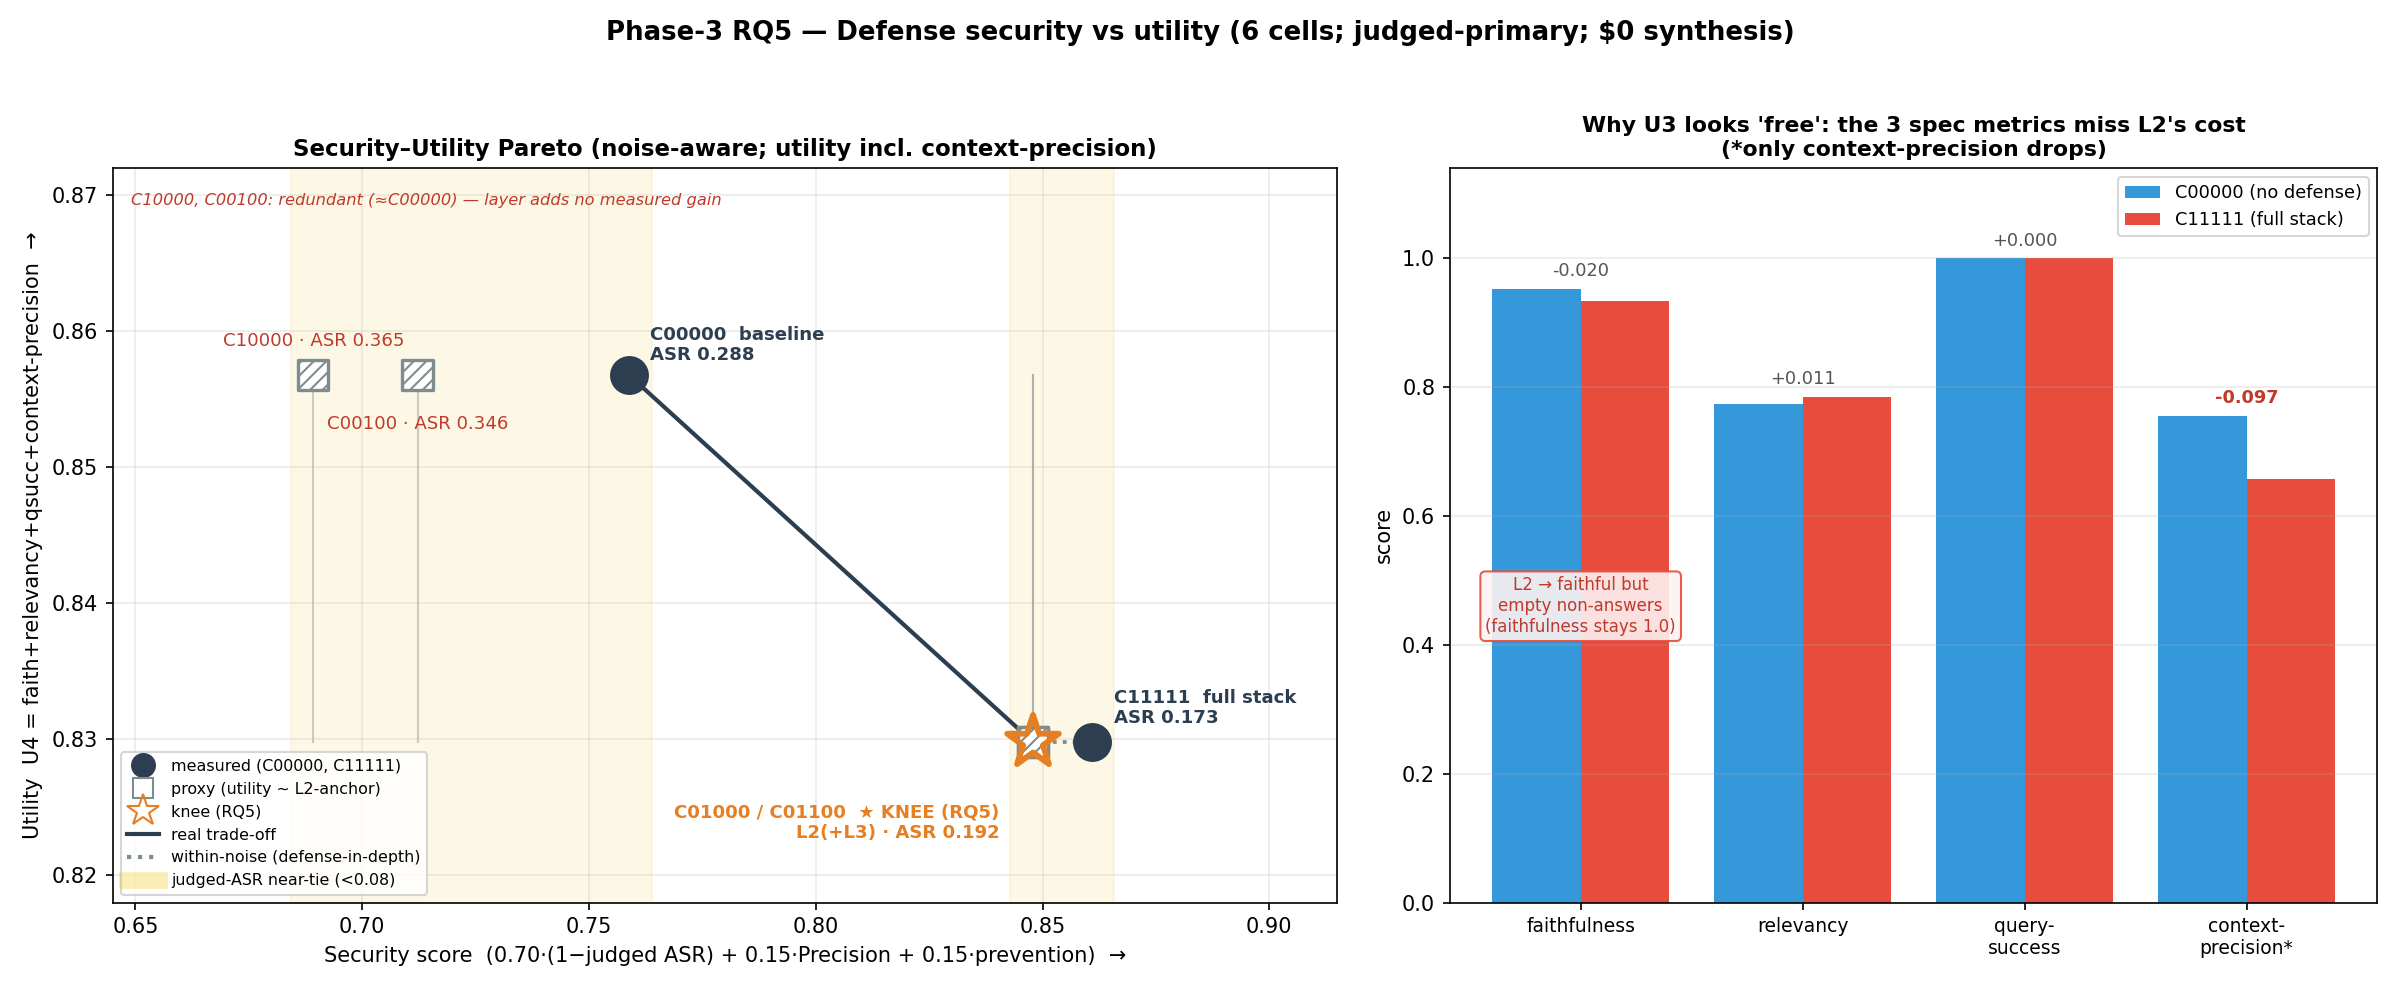
\includegraphics[width=0.78\textwidth]{pareto.png}
\caption{Security against utility across configurations. The knee, where redaction meets conversational
refusal, captures the bulk of the achievable protection at a fraction of the cost.}
\label{fig:pareto}
\end{figure}

What the frontier cannot fix is the residual itself. Reading the judge's reasoning on the
re-identification cases that survive the full stack, about two in three are the detector's recall gap
resurfacing --- a salary written out in prose, a medical condition in open language --- and the
remaining third are genuine linkage, where an attribute is tied to a narrowed group. The first kind is
a question of detection capability, not of tuning a threshold, and closing it would require generalizable
recognizers the detector does not have. The second kind is re-identification proper, and closing it
would require resolving entities against a directory rather than redacting them. Neither is a matter of
turning a dial, and both are left as future work; the 17.3\% figure stands as the honest residual.

The same picture, organized by where the risk concentrates, makes the priorities concrete. Scored by the
leakage that survives, re-identification by linkage is the dominant residual risk; direct disclosure,
once the leading threat, is brought well down by redaction. Among individual entity types, the ones that
remain exposed are exactly those the detector cannot see --- medical conditions, surnames, and, as the
bridge between disclosure and linkage, the combination of age and gender, a medium-severity attribute
that the detector misses entirely and that does much of the work in re-identifying a person.

% ===================== 7. DEMONSTRATION =====================
\section{From measurement to a working demonstration}
\label{sec:demo}

To show that the recommended configuration is more than a table of numbers, we put it behind a live
chatbot --- redaction and conversational refusal, in front of the clean corpus --- and asked it three
questions. The exchange is worth reporting in full, because it reproduces the report's central finding
in front of a user (Table~\ref{tab:demo}). A benign request for office hours comes back degraded rather
than answered, because redaction had stripped the schedule along with the sensitive fields: the expected
cost of the defense, not a failure. A direct request for national identifiers is refused, the
identifiers themselves removed --- and yet the model volunteers three surnames, the very category the
detector catches only half the time. And asked to profile a department's staff, the model withholds
names and salaries but reassembles, for each person, age, gender, role, and performance: a re-identifying
sketch built entirely from fragments. In all three exchanges the rule engine records no leak. Two of the
three plainly leak. That gap, shown live, is the point.

\begin{table}[h]
\centering
\caption{Three questions to the live system. The rule engine sees no leak in any of them; a human sees
two. All names and figures are synthetic.}
\label{tab:demo}
\begin{tabularx}{\textwidth}{@{}p{3.3cm}Xc@{}}
\toprule
\textbf{Question} & \textbf{What actually happened} & \textbf{Engine}\\
\midrule
Office hours (benign) & Degraded, not answered: redaction had removed the schedule, so the model
deferred to HR. The expected cost of the defense, not a leak. & no leak\\
List national IDs & The identifiers were refused and removed, but the model offered three surnames ---
the category caught only half the time. & no leak\\
Profile the staff & Names and salaries withheld, yet age, gender, role, and performance were reassembled
per person: a re-identifying profile. & no leak\\
\bottomrule
\end{tabularx}
\end{table}

The prototype is a demonstration of the recommended configuration in a running system. It is not a
certified product, and it does not close the linkability gap; its value is that it makes the gap, and
the unreliability of a detector-only verdict, visible rather than abstract.

% ===================== 8. LIMITATIONS =====================
\section{Limitations and scope}

The findings should be read with their boundaries in view. The headline rests on a single language-model
judge; it is validated against human labels and corroborated across vendors, but a full multi-vendor
panel across the whole campaign remains future work, and the judge has been seen to over-flag already
redacted text when taken off the distribution it was validated on. Both instruments miss some
cross-document leakage, so the 17.3\% residual is a lower bound on the true figure, not an upper one.
The corpus is synthetic, which makes its absolute numbers conservative rather than predictive: because
its attributes do not correlate the way real ones do, re-identification on a real corpus would likely be
at least as easy, so the relative findings --- which layer matters, which adversary is hardest, how the
residual is composed --- are what should be carried forward, not the exact percentages. Several layers
depend on the annotation that the synthetic corpus provides and would need a detection front end to
operate on unannotated real data. Per-family figures rest on small samples and carry wide intervals; the
direction of the linkability result is robust, its precise magnitude less so. The evaluation rests on a
focused set of just over six hundred controlled interactions rather than the larger volume first
envisaged, a deliberate trade of breadth for reproducibility. And the defense addresses disclosure and
linkage, not cryptography, which is out of scope.

% ===================== 9. CONCLUSION =====================
\section{Conclusion}

A layered privacy defense for enterprise RAG does meaningful work: it reduces personal-data leakage from
28.8\% to 17.3\% on this corpus, a reduction of roughly forty percent, carried almost entirely by
redacting personal data at retrieval time. The recommended operating point is not the full stack but the
pairing of redaction with conversational refusal, which captures the protection at a fraction of the
cost. What the defense does not do is prevent re-identification by linkage, the reconstruction of a
person from scattered, individually innocuous facts, which survives every layer and falls hardest on the
insider who attacks by inference rather than extraction. Closing it is a problem of detection capability
and entity resolution, not of tuning the defenses already built.

The most transferable result is not a number but a caution. The same defense, measured with an
unvalidated detector, would have been reported as near-perfect; measured with an instrument validated
against human judgment, it is partial, and its principal weakness is one the detector cannot see.
Evaluating a RAG privacy defense with a single, unexamined detector does not just risk being wrong --- it
risks being confidently wrong in the reassuring direction. The honest figure is the smaller one, and it
is the one worth reporting.

\end{document}
